\section{Numerical Methodology}
% From TOFE 2014
Researchers of ceramic pebble beds for fusion reactors are concerned with damage to individual pebbles in the solid breeder volume; the accumulation of damage (\textit{e.g.} sintering, crushing) to many pebbles will ultimately have global effects on the tritium performance of the pebble bed volume.  The discrete element method provides us with the ability to probe particle-scale interactions so that we might understand, predict, and more importantly, avoid pebble damage and the morphological changes to the pebble bed associated with it. However, simulations with the DEM alone are only telling half of the story of the solid breeder. DEM models (as we are implementing them) are not able to capture the effects, neither on momentum nor energy, of an interstitial fluid. Therefore we present a modeling technique to supplement the DEM computations with a volume-averaged thermofluid model of helium (we will frequently refer to the thermofluid model as the computational fluid dynamics (CFD) method). The technique of coupling CFD to DEM was first proposed by Tsuji\etal.\cite{Tsuji1992} in 1992. Since that time, the CFD-DEM coupling approach has grown as a tool for granular flow research. A comparison of model formulation for CFD-DEM is discussed clearly by Zhou\etal\cite{Zhou2010}.

\subsection{Helium in the DEM Framework}\label{sec:cfdem-heat-transfer}

The numerical framework behind the discrete element was given in \cref{sec:particle-dynamics}. In the DEM model, each pebble obeys Newton's equations of motion. As the fluid passes through the packed bed of pebbles, it imparts a force on each individual pebble which cumulatively total to the pressure drop across the bed. To include the influence of helium, we simply augment the the linear momentum of Eq.~\ref{eq:newton-translational} to include the drag force of the fluid on the particle. The momentum balance of our Lagrangian-tracked pebble now reads,
\begin{equation}\label{eq:cfdem-dem-momentum}
	m_i  \ddt{\vec{r}_i} = m_i\vec{g} + \vec{f}_i + \beta_i V_i \Delta u_{if}
\end{equation}
where all but the last term is identical to Eq.~\ref{eq:newton-translational} but the last term accounts for the fluid. $\Delta u_{if} = u_f - u_i$, is the relative velocity between the fluid and pebble, $i$, and the inter-phase momentum exchange coefficient, $\beta_i$, acts upon the entire pebble volume, $V_i$. 

Similarly, as the helium of temperature $T_f$ passes over the particle at temperature $T_i$, energy will be exchanged. For consistency with the momentum equation, we introduce an inter-phase energy exchange coefficient (a renaming of the heat transfer coefficient) which we assume to be constant for the entire surface of the particle. The energy balance of the particle was given in Eq.~\ref{eq:thermoFirstLaw}. After adding the inter-phase energy exchange coefficient, it now reads,
\begin{equation}\label{eq:cfdem-dem-energy}
	m_iC_i \ddt{T_i} = Q_{s,i} + \sum_{j=1}^Z Q_{ij} + \beta_{E,i} A_i \Delta T_{if}
\end{equation}
where again we have only needed to add the last term to account for the energy deposited/removed by the fluid. $\Delta T_{if} = T_f - T_i$, and the inter-phase energy exchange coefficient, $\beta_{E,i}$, acts upon the pebble surface area, $A_i$.

These simple additions to the governing equations of momentum and energy of each particle are all that are necessary to introduce helium into the DEM computations. The difficulty arises in the computation of the inter-phase exchange coefficients, $\beta_i$ and $\beta_{E,i}$. We will discuss their calculations next.

\subsection{Inter-phase Exchange Coefficients}
In \cref{sec:modeling-pressure-drop}, we showed a number of correlations that engineers use to calculate the pressure drop in packed beds of spheres. The purge gas in ceramic breeders is meant to travel at very low flow rates to maximize the absorption of tritium. Furthermore, the pebble beds will always be near the close-packed limit. As such, the particle Reynolds number for these flows is often near unity and the Kozeny-Carman equation as applicable for Stokes flow is quite sufficient (see the assumptions leading to Eq.~\ref{eq:K-C-non-dim}). However, the Koch-Hill-Ladd correlation of Eq.~\ref{eq:khl-correlation} which includes terms for both the Stokes flow correlation (as a function of $\phi$) in the zero-Reynolds number limit and the viscous effects with a Reynolds number-dependent term is a general correlation that reduces to the Kozeny-Carman correlation in the close-packed, zero-Reynolds number limits. Thus for our model, we implement the KHL correlation.

The inter-phase momentum exchange coefficient is simply a re-writing of the non-dimensional drag force from Eq.~\ref{eq:khl-correlation}. The common form by Gidaspow\cite{gidaspow1994multiphase} differs from what we use here by a factor of $1-\phi$ due to definitions of the drag force. We use the form from Koch, Hill, \& Ladd.\cite{Hoef2005,Benyahia2006}
\begin{equation}\label{eq:interphase-momentum}
	\beta_{i} = \frac{18\mu_f}{d_{p,i}^2}(1-\phi_k)\phi_k F
\end{equation}
where $\mu_f$ is the fluid viscosity and the diameter of pebble $i$ is $d_{p,i}$. The packing fraction, $\phi_k$, in this equation is the local packing fraction in the fluid cell $k$. This value will differ from the global/bulk value in near-wall regions. Container walls have long been known to theoretically and experimentally force order to the packing regardless of shape of packing.\cite{Hunt1990,Benenati1962,Baird1958} For example, the void fraction ($\epsilon = 1-\phi$) in narrow annular containers using the correlation from Mueller, as a function of wall-distance in a cylinder is,\cite{Mueller1999}
\[
\epsilon = \epsilon_0 + (1-\epsilon_0)J_0(ar^*)e^{-br^*}
\]
where $r^*$ is the non-dimensional distance from the wall; here it is defined in terms of the pebble diameter, $r^* = r/d_p$. The constants, a and b, are defined in terms of the size parameter $\alpha = D/d_p$ where $D$ is the diameter of the annular tube. First, $a$ is
\[
    a= 
\begin{cases}
    7.383 - \cfrac{2.932}{\alpha - 9.864}, & \text{if }~ \alpha \geq 13\\
    8.243 - \cfrac{12.98}{\alpha + 3.156}, & \text{if} ~13 \geq \alpha \geq 2.61
\end{cases}
\]
then
\[
b = 0.304 - \cfrac{0.724}{\alpha}
\]
The bulk void fraction is found from the correlation:
\[
\epsilon_0 = 0.379 + \cfrac{0.078}{\alpha - 1.8}
\]

We then plot the packing fraction as a function of distance from the container wall for two example sizes, diameters of 20$d_p$ and 5$d_p$, in Fig.~\ref{fig:packingDist}. This example is meant to demonstrate the varying packing fraction in a packed bed that is described with a bulk or global packing fraction. The size of the discretized cell relative to the pebble will dictate how much of the void fraction variation is captured in the volume-averaged equations.

\begin{figure}[htbp]
\begin{center}
	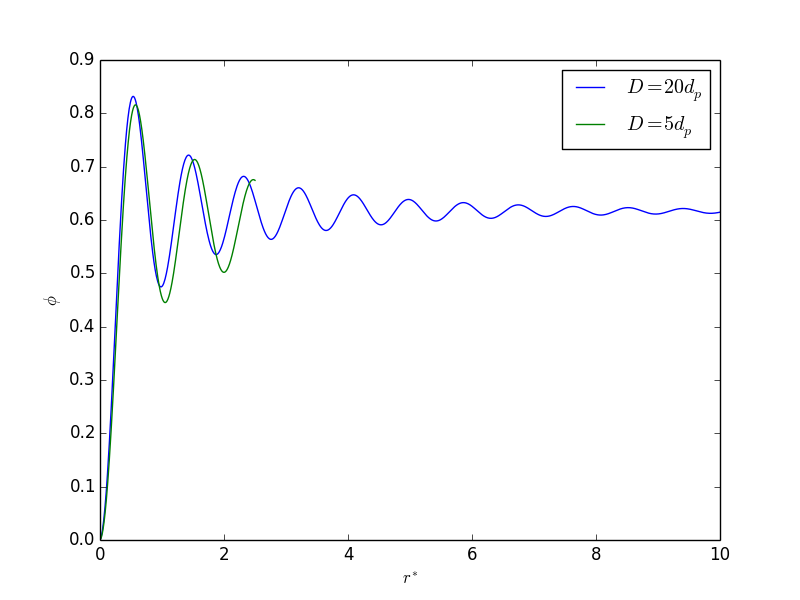
\includegraphics[width = \singleimagewidth]{chapters/figures/annular-packing-fraction.png}
	\caption{Showing the packing fraction approach the bulk value after a few pebble diameters when the pipe is 20$d_p$ and that when the pipe is only 5$d_p$, the packing fraction at any radius is not the same as the bed average.}
	\label{fig:packingDist}
\end{center}
\end{figure}
\FloatBarrier


The inter-phase energy transfer coefficient is of the same form as a traditional heat transfer coefficient and is likewise calculated from the Nusselt number for the helium flow.
\begin{equation}\label{eq:interphase-energy}
	\beta_{E,i} = \frac{\Nu k_f}{d_{p,i}}
\end{equation}
where $k_f$ is the thermal conductivity of the fluid. Several correlations for determining the Nusselt number were given in \cref{sec:particle-convection}. We opt for the correlation provided by Li \& Mason.\cite{Li2000} Which is applicable to a wide range of Reynolds number flows [and packing fractions?].

From Eqs.~\ref{eq:interphase-momentum} and~\ref{eq:interphase-energy}, we have a formulation wherein knowledge of the flow field around our pebbles will allow calculation of dimensionless drag, $F$, and Nusselt number, $\Nu$, and the flow is coupled to our DEM computations with simple additions to the equations of motion and energy of the pebble. We next 




\subsection{Volume-averaged Thermofluid Flow}

The gas phase flow field will be treated with volume-averaging theory (VAT).\cite{Sbutega2013,whitaker1999method,Tsuji1992} The VAT allows treatment of complex porous flows with smooth continuous equations. In the VAT, we average over a discrete space to replace complex geometry with a fictitious, smooth, continuous medium in which quantities of interested are defined independently of whether specific locations in that space are, for instance, solid or gas.

In this formulation of the gas flow, we discretize the gas space with cells that are much larger than the individual particles; in the application of our CFD-DEM coupling, this meant approximately 5~6 particles per cell. With VAT, the particles themselves are not resolved in the fluid space but are simply introduced via closure terms.\cite{Sbutega2013,Horvat2006} Derivation of the governing equations of VAT can be found in Sbutega \& Catton\cite{Sbutega2013}. The momentum and energy of a fluid flow through a solid phase with volume-averaged Navier-Stokes and energy equations are applied to each cell, $k$, in the discretized fluid space,
\begin{subequations}
\begin{align}
\pder[\epsilon_k \rho_f]{t} + \nabla\cdot(\epsilon_k u_f \rho_f) &= 0\\
\pder[\epsilon_k u_f]{t} + \nabla\cdot(\epsilon_k u_f u_f) &= -\frac{\epsilon_k}{\rho_f}\nabla P_f + \nabla\cdot\left(\nu_f\epsilon_k\nabla u_f\right) - \frac{S_k}{\rho_f}\\
\pder[\epsilon_k T_f]{t} + \nabla\cdot(\epsilon_k u_f T_f) &= \nabla\left(\epsilon_k\epsilon\nabla T_f\right)-\frac{E_k}{\rho_fC_f}
\end{align}
\end{subequations}

The packing fraction in any fluid cell is calculated by summing through all the volumes of $k$ particles located in that cell
\begin{equation}
	\phi_k = \sum_{i=1}^k \frac{V_{p,i}}{\Delta V_k}
\end{equation}
where the fluid void fraction is the complement of the solid packing fraction, $\epsilon = 1 - \phi$. 

Coupling the fluid phase to the particles happens with the sink terms in momentum and energy of $S_k$ and $E_k$, respectively. They are volume-weighted sums of the drag forces and energy exchanges, respectively, for all particles in the discretized fluid cell,
\begin{subequations}
\begin{align}
	S_k &= \frac{1}{V_k}\sum_{\forall i \in k} \beta_i V_i \Delta u_{if}\\
	E_k &= \frac{1}{V_k}\sum_{\forall i \in k} \beta_{E,i} A_i \Delta T_{if}
\end{align}
\end{subequations}
The inter-phase momentum and energy exchange coefficients act as the communicators between the particle information from the DEM solver and the fluid fields from CFD. Thus the motion and energy of the fluid field are intimately coupled with the particle positions and energy, but computational time is preserved by only considering volume-averaged values in the fluid domain. %The cross-communication between fluid and solid is accomplished with a coupling routine that is explained in detail in Refs. 11, 12.


\subsection{Discussion of Methodology}
Discussion of three sets of governing equations\cite{Zhou2010}
Since the introduction of the CFD-DEM coupling methodology by Tsuji\etal~in 1993 and then Hoomans\etal~in 1996, many researchers have adopted the approach when particle-scale information of granular and fluidized beds is important.\cite{Tsuji1993,Hoomans1996} Fluidized beds have many industrial applications and are most often studied with coupled CFD-DEM tools. Review papers \cite{Zhu2007} and \cite{Deen2007}